%===== Chapter 2: Requirements Analysis =====%

\chapter{Requirements Analysis}

\section*{Introduction}
This chapter identifies the platform actors, documents the functional and
non-functional requirements, and presents selected use case descriptions.

\section{Actors Identification}

The platform involves four distinct actor types:

\begin{longtable}{|m{3.5cm}|m{10cm}|}
    \hline
    \textbf{Actor}      & \textbf{Description}                                                                                                                                                                        \\
    \hline
    \endhead
    \endfoot
    \endlastfoot
    \hline
    Guest Visitor       & An anonymous user browsing the storefront. Their session is tracked server-side to persist a basket, manage a wishlist, apply coupons, and place orders without requiring account creation. \\
    \hline
    Registered Customer & A visitor who has created an account. They can log in, track order status, and manage placed orders.                                                                                        \\
    \hline
    Administrator       & A privileged backoffice user who manages the catalog, promotions, CMS, and site configuration.                                                                                              \\
    \hline
    Super Administrator & An administrator with the highest privilege level, able to manage selling points and admin accounts.                                                                                        \\
    \hline
    Cashier             & An admin role assigned to a physical selling point, responsible for processing in-store POS sales, viewing the catalog, managing orders, generating invoices, and issuing credit notes.     \\
    \hline
    \caption{Platform actors}
    \label{tab:actors}
\end{longtable}

\section{Functional Requirements}

\subsection{Authentication and Account Management}

\begin{itemize}
    \item \textbf{FR-AUTH-01:} A visitor can register an account with name, email, password, and phone number.
    \item \textbf{FR-AUTH-02:} A registered user can log in and receive a signed JWT token.
    \item \textbf{FR-AUTH-03:} An anonymous visitor receives a server-managed session cookie on first visit, enabling guest basket persistence.
    \item \textbf{FR-AUTH-04:} An administrator or cashier can log in through a dedicated admin login page.
    \item \textbf{FR-AUTH-05:} The super admin account is created via a one-time seed script.
    \item \textbf{FR-AUTH-06:} Password reset flow is available for both customers and admins.
\end{itemize}

\subsection{Product Catalog}

\begin{itemize}
    \item \textbf{FR-CAT-01:} Products are organised in a three-level taxonomy: Category $\rightarrow$ Subcategory $\rightarrow$ Product.
    \item \textbf{FR-CAT-02:} Products can be associated with a Brand.
    \item \textbf{FR-CAT-03:} Each product has a name, slug, description, price, discount price, images, and stock.
    \item \textbf{FR-CAT-04:} Stock is tracked per product.
    \item \textbf{FR-CAT-05:} Products support barcode lookup via the GO\_UPC API.
    \item \textbf{FR-CAT-06:} A product can optionally have an associated 3D model for in-browser preview.
    \item \textbf{FR-CAT-07:} Administrators can create, update, publish/unpublish, and delete any catalog entity.
    \item \textbf{FR-CAT-08:} Products support full-text search on both the storefront and admin.
\end{itemize}

\subsection{Shopping and Commerce}

\begin{itemize}
    \item \textbf{FR-COM-01:} Any visitor (guest or registered) can add products to a basket, update quantities, and remove items.
    \item \textbf{FR-COM-02:} Any visitor can place an order from their basket, providing a delivery address and selecting a governorate.
    \item \textbf{FR-COM-03:} Orders progress through a defined status lifecycle: \texttt{pending $\rightarrow$ confirmed $\rightarrow$ processing $\rightarrow$ shipped $\rightarrow$ delivered $\rightarrow$ cancelled}.
    \item \textbf{FR-COM-04:} Registered customers can track order status and manage their placed orders from their account dashboard.
    \item \textbf{FR-COM-05:} Cashiers and Administrators can view, filter, search, and update the status of all orders.
    \item \textbf{FR-COM-06:} Any visitor can maintain a wishlist of saved products.
    \item \textbf{FR-COM-07:} Shipping rates are configurable per governorate or delivery zone.
\end{itemize}

\subsection{Promotions and Coupons}

\begin{itemize}
    \item \textbf{FR-PROMO-01:} Administrators can create promotional campaigns and coupon codes that apply to specific products, categories, subcategories, brands, or all items.
    \item \textbf{FR-PROMO-02:} Promotions can be of different types: percentage discount, ``buy X get Y'', or ``buy 1 get another product for free''.
    \item \textbf{FR-PROMO-03:} Administrators can create coupon codes with usage limits, expiry dates, and the same target and type rules as promotions.
    \item \textbf{FR-PROMO-04:} Any visitor can apply a coupon code at checkout, and the system tracks usage to enforce limits.
\end{itemize}

\subsection{Invoicing and Financial Documents}

\begin{itemize}
    \item \textbf{FR-INV-01:} The system auto-generates a sequential invoice number for every confirmed order.
    \item \textbf{FR-INV-02:} Administrators and Cashiers can generate PDF invoices for any order or create manual invoices.
    \item \textbf{FR-INV-03:} Administrators and Cashiers can issue credit notes (partial or full refund documents) linked to an invoice.
    \item \textbf{FR-INV-04:} Credit note PDFs are downloadable from the backoffice.
\end{itemize}

\subsection{Content Management System (CMS)}

\begin{itemize}
    \item \textbf{FR-CMS-01:} Administrators can publish, edit, and delete blog articles.
    \item \textbf{FR-CMS-02:} Blog articles are publicly accessible on the storefront.
    \item \textbf{FR-CMS-03:} Administrators can manage promotional banners displayed on the homepage.
    \item \textbf{FR-CMS-04:} Site-wide configuration (store name, contact info, social links, SEO metadata) is managed via a single site-config form.
    \item \textbf{FR-CMS-05:} Image uploads are handled server-side with automatic optimisation (Sharp).
\end{itemize}
\subsection{Selling Points Management}

\begin{itemize}
    \item \textbf{FR-SP-01:} A selling point represents a commercial entity, which can be the main website or a physical store location.
    \item \textbf{FR-SP-02:} The Super Administrator can create, update, and delete selling points.
    \item \textbf{FR-SP-03:} The Super Administrator can assign a Cashier role to a specific physical selling point.
    \item \textbf{FR-SP-04:} Cashiers can manage sales and operations only within their assigned physical selling point.
    \item \textbf{FR-SP-05:} Cashiers can browse the product catalog and search for products via text or barcode scanning.
    \item \textbf{FR-SP-06:} Cashiers can add products to a local basket and process in-store point-of-sale (POS) orders.
\end{itemize}

\subsection{Customer Support}

\begin{itemize}
    \item \textbf{FR-SUP-01:} Customers can open a support ticket from the storefront.
    \item \textbf{FR-SUP-02:} Real-time messaging between customers and support staff is provided via WebSocket (Socket.IO).
    \item \textbf{FR-SUP-03:} Support tickets are mirrored to a Discord channel via a Discord bot, enabling the team to respond from Discord.
    \item \textbf{FR-SUP-04:} Ticket status tracking (open, in-progress, resolved, closed) is available in the backoffice.
\end{itemize}

\subsection{Notifications and Locations}

\begin{itemize}
    \item \textbf{FR-NOTIF-01:} Transactional emails (order confirmation, registration, password reset) are sent via SMTP (Nodemailer).
    \item \textbf{FR-LOC-01:} The system stores all 24 Tunisian governorates as reference data.
    \item \textbf{FR-LOC-03:} Delivery fees can be configured per governorate.
\end{itemize}

\section{Non-Functional Requirements}

\begin{longtable}{|m{1.5cm}|m{2.5cm}|m{9cm}|}
    \hline
    \textbf{ID} & \textbf{Category} & \textbf{Requirement}                                                                                 \\
    \hline
    \endhead
    \endfoot
    \endlastfoot
    \hline
    NFR-01      & Security          & All sensitive routes require authentication. JWT tokens are short-lived and signed with a secret.    \\
    \hline
    NFR-02      & Security          & Passwords are hashed with bcrypt. No plaintext credentials in the database.                          \\
    \hline
    NFR-03      & Security          & HTTP headers hardened with Helmet. CORS restricted to configured origins.                            \\
    \hline
    NFR-05      & Security          & CI/CD runs Trivy security scans on both filesystem and built Docker images (CRITICAL/HIGH blocking). \\
    \hline
    NFR-06      & Performance       & Next.js SSR/SSG ensures fast first-paint and good Core Web Vitals on the storefront.                 \\
    \hline
    NFR-07      & Performance       & MongoDB indexes on frequently queried fields (slug, category, status).                               \\
    \hline
    NFR-08      & Availability      & Zero-downtime deployments via rolling update + health check polling. Automatic rollback on failure.  \\
    \hline
    NFR-09      & Availability      & Auto-healing script restarts unhealthy containers and sends Discord alerts.                          \\
    \hline
    NFR-10      & Scalability       & Stateless API (sessions in MongoDB, files on a mounted volume) allows horizontal scaling.            \\
    \hline
    NFR-11      & Maintainability   & NestJS module system enforces separation of concerns.                                                \\
    \hline
    NFR-12      & Usability         & Storefront is fully responsive (mobile-first Tailwind CSS).                                          \\
    \hline
    NFR-13      & Observability     & Netdata monitors CPU, memory, disk, and container health with alerting.                              \\
    \hline
    \caption{Non-functional requirements}
    \label{tab:nfr}
\end{longtable}

\section{Use Case Diagrams}

\begin{figure}[H]
    \centering
    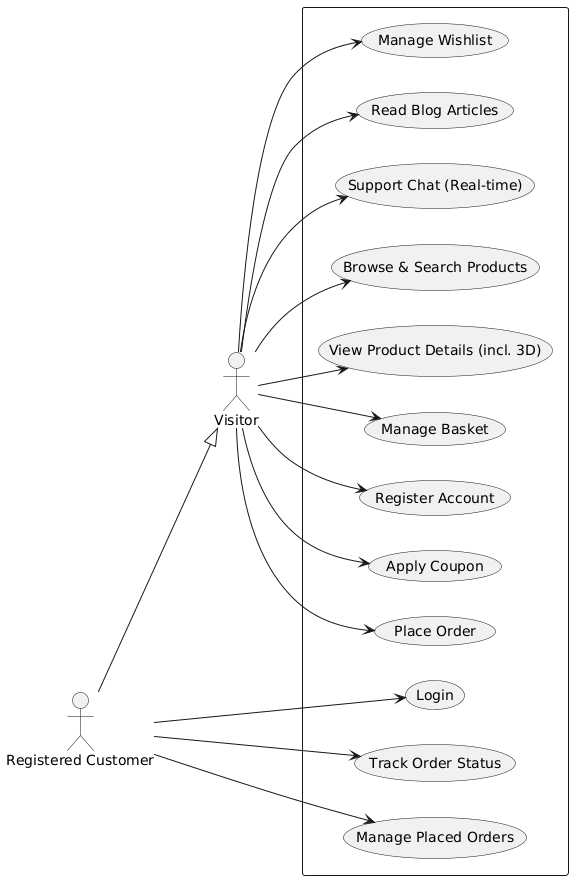
\includegraphics[width=\textwidth,height=0.45\textheight,keepaspectratio]{img/usecaseVistor.png}
    \caption{Customer use case diagram}
    \label{fig:uc_customer}
\end{figure}

\begin{figure}[H]
    \centering
    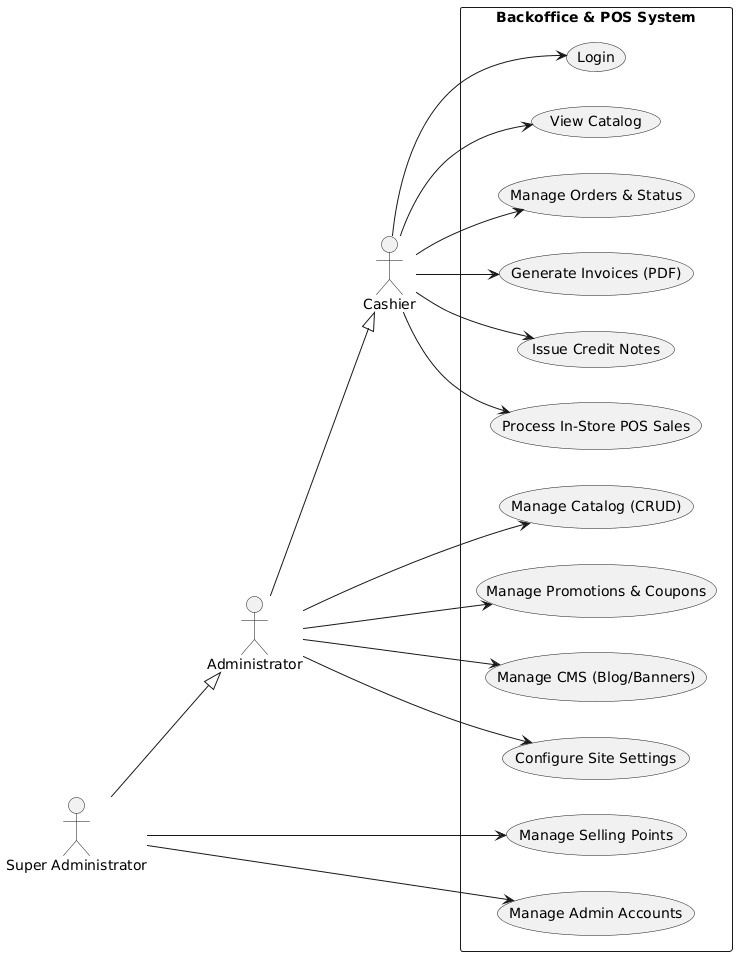
\includegraphics[width=\textwidth,height=0.45\textheight,keepaspectratio]{img/usecaseAdmin.png}
    \caption{Administrator use case diagram}
    \label{fig:uc_admin}
\end{figure}

\section{Selected Use Case Descriptions}

\subsection{UC-01: Place an Order}

\begin{longtable}{|m{3.5cm}|m{10cm}|}
    \hline
    \textbf{Field}   & \textbf{Detail}                                                                                                                                                                                                                                                                                                                                                                \\
    \hline
    \endhead
    \endfoot
    \endlastfoot
    \hline
    Actor            & Visitor                                                                                                                                                                                                                                                                                                                                                                        \\
    \hline
    Precondition     & Basket contains at least one item                                                                                                                                                                                                                                                                                                                                              \\
    \hline
    Main Flow        & 1. Visitor navigates to cart. 2. Clicks ``Proceed to Checkout''. 3. System displays checkout form. 4. Visitor submits the form. 5. System validates stock, calculates shipping, applies coupon if present. 6. System creates an order with status \texttt{pending}. 7. Clears the basket. 8. Sends order confirmation and acount creation email. 9. Redirects to success page. \\
    \hline
    Alternative Flow & If a product is out of stock, the system returns a 400 error and the order is not created.                                                                                                                                                                                                                                                                                     \\
    \hline
    Postcondition    & Order exists in the database.                                                                                                                                                                                                                                                                                                                                                  \\
    \hline
    \caption{UC-01: Place an Order}
    \label{tab:uc01}
\end{longtable}

\subsection{UC-02: Issue a Credit Note}

\begin{longtable}{|m{3.5cm}|m{10cm}|}
    \hline
    \textbf{Field} & \textbf{Detail}                                                                                                                                                                                \\
    \hline
    \endhead
    \endfoot
    \endlastfoot
    \hline
    Actor          & Cashier (and Administrator)                                                                                                                                                                    \\
    \hline
    Precondition   & An invoice exists for the order                                                                                                                                                                \\
    \hline
    Main Flow      & 1. Admin opens the invoice. 2. Selects ``Issue Credit Note''. 3. Specifies items to credit and reason. 4. System generates a credit note with a sequential number. 5. Admin downloads the PDF. \\
    \hline
    \caption{UC-02: Issue a Credit Note}
    \label{tab:uc02}
\end{longtable}

\section*{Conclusion}
This chapter identified four distinct actors and documented over 30 functional
requirements across 10 functional domains, together with 13 non-functional requirements
covering security, performance, availability, and maintainability. The following
chapter translates these requirements into a concrete system design.
